\documentclass[10pt,executivepaper]{article}
\usepackage[utf8]{inputenc}
\usepackage[spanish]{babel}
\usepackage{amsmath}
\usepackage{amsfonts}
\usepackage{amssymb}
\usepackage{graphics}
\usepackage{graphicx}
\usepackage[left=2cm,right=2cm,top=2cm,bottom=2cm]{geometry}
\usepackage{imakeidx}
\makeindex[columns=3, title=Alphabetical Index, intoc]
\usepackage{listings}
\usepackage{xcolor}
\usepackage{multicol}
\usepackage{changepage}
\usepackage{float}
\usepackage{cite}
\usepackage{url}
\usepackage{hyperref}

\definecolor{codegreen}{rgb}{0,0.6,0}
\definecolor{codegray}{rgb}{0.5,0.5,0.5}
\definecolor{codepurple}{rgb}{0.58,0,0.82}
\definecolor{backcolour}{rgb}{0.95,0.95,0.92}

\lstdefinestyle{mystyle}{
    backgroundcolor=\color{backcolour},
    commentstyle=\color{codegreen},
    keywordstyle=\color{magenta},
    numberstyle=\tiny\color{codegray},
    stringstyle=\color{codepurple},
    basicstyle=\ttfamily\footnotesize,
    breakatwhitespace=false,
    breaklines=true,
    captionpos=b,
    keepspaces=true,
    numbers=left,
    numbersep=5pt,
    showspaces=false,
    showstringspaces=false,
    showtabs=false,
    tabsize=3
}

\lstset{style=mystyle}

\title{Lenguaje C\\Curso de programación en C\\Escuela Superior de Cómputo}

\author{A cargo del profesor: Cristhian Avila Sanchez\\Escrito por: Adrian González Pardo}

\date{\today}

\newcommand\tab[1][1cm]{\hspace*{#1}}

\begin{document}
% Portada
%encabezado
\begin{minipage}{0.4\textwidth}
	\begin{flushleft}
		
\includegraphics[scale = 0.05]{logoescom.png}
	\end{flushleft}
\end{minipage}
\begin{minipage}{0.51\textwidth}
	\begin{flushright}
		
\includegraphics[scale = 0.055]{logoipn.png}
	\end{flushright}
\end{minipage}
\begin{center}
	\par\vspace{0.5cm}{
	\huge\textbf{Instituto Politécnico Nacional \\*[0.20cm] Escuela Superior de Cómputo}}
\par\vspace{1cm}{
	\large\textbf{Lenguaje C\\Curso de programación en C\\A cargo del profesor: Cristhian Avila Sanchez\\Escrito por: Adrian González Pardo\\}
}
\par\vspace{1cm}{
	
\includegraphics[scale=1.5]{lenguaje-c.png}
}
\par\vspace{2cm}{
	Ultima fecha modificado: \today
}
\end{center}

% Indice
\clearpage
\tableofcontents
\clearpage

%Contenido
\section{Compilación algunos sistemas operativos}
En algunos de los casos más comunes el intentar compilar a nivel consola (CMD, Terminal) es en algunos casos un tabu para los iniciados en la progración o que simplemente se han apoyado de IDE's que les permiten evitarse esta tarea en las cuales si bien en un trabajo rapido, es necesario tambien poder trabajar con este compilador a nivel consola, por lo cual se puede hacer de la siguiente forma en los siguientes sistemas operativos.
\subsection{Linux}
Si bien el compilador de lenguaje C viene nativamente en los binarios y utilerias del sistema del proyecto Linux y GNU/Linux en algunos casos podemos no encontrar el compilador de lenguaje C (GCC), por lo cual acorde al sistema de empaquetamiento que se maneje en sus sistemas Linux es necesario instalar el paquete gcc, gcc-multilib.\\
Para el caso de sistemas basados en Debian con empaquetamiento deb y que soporten apt-get, apt se sigue las siguentes líneas de comandos.\\
\tab \textit{\$\_ sudo apt install build-essential gcc gcc-multilib -y}
\subsection{MacOS}
En el caso de ser un sistema operativo MacOS, es necesario tomar encuenta en que las siguientes líneas de comandos puede funcionar o no, por lo cual en caso de que exista algun error es necesario buscar la versión compatible con el sistema operativo que tengan de base\\
\tab \textit{\$\_ sudo port install gcc48\\
\tab\$\_ sudo port select -set gcc mp-gcc48}
\subsection{Windows}
Para ultimo caso en un sistema de Windows es necesario bajar el compilador e instalarlo o en su defecto se puede bajar el IDE Codeblocks con el compilador, Dev C o Dev C++, una vez realizada la instalación de alguno de estos IDE's es necesario conocer la ruta de instalación de la aplicación, por lo cual se ira hasta su localización, donde generalmente el compilador en estas aplicaciones esta resguardado en la subcarpeta de ./bin/ , por lo cual copiaremos la ruta completa que este en la navegación, posteriormente en la barra de inicio se buscara "Variables de Entorno", una vez en este apartado en las variables se buscara el apartado de la variable "PATH" en la cual se modificara y a no remplazando el contenido de esta previamente con ";" en el caso de que sea un string continuo se pegara la ruta (ejemplo) [/ruta/ruta/ideDePreferencia/bin/] y en caso de que no sea un string continuo solo se añadira esto y asi a traves de CMD o PowerShell se puede hacer uso del compilador gcc
\subsection{Compilación desde consola}
Si bien ya conocemos el como se instala el compilador de lenguaje C para usarlo a nivel consola, ahora un uso generico sin necesidad de quebrarse la cabeza es la compilación rapida de archivos C
\\
\tab \textit{\$\_ gcc $<$archivo de extensión c$>$}\\
Para conocer más opciones acerca de lo que puede o no hacer el binario gcc, tenemos:\\
\tab \textit{\$\_ gcc --help}
\section{Pointers (Apuntadores)}
Es una entidad de referencia a otras zonas de memoria, estos hacen una referencía a una variable de un tipo de dato básica (\textit{int, float, long, byte, short})
\\
Un ejemplo de como se escriben estos apuntadores en la lógica del lenguaje C es\\
\tab \textit{int *p = NULL, \\\tab x=0;}\\
De este modo podemos imaginar que se asigna una sección de memoria en estos ambos casos los cuales a nivel memoria contendran dos direcciones distintas lo cual para terminos de ejemplificación se asignara las siguientes secciones de memoria para las variables\\
\tab \emph{p = 0x006 , x = 0xAF32}\\
Ahora una vez que sabemos que de esta forma se asignan las secciones de memoria, hacemos uso de la asignación de dirección de memoria de la variable x a la variable p, es decir que podamos hacer via apuntador de la memoria sin necesidad de llegar a la seccion de la variable x\\
\tab \textbf{p = \&x; \\//Lo cual quiere decir que la dirección del apuntador p esta directamente relacionada a la sección donde habita x sin que exista una forma de apuntar de forma inversa}
\subsection{Un poco de brevario a la simbologia \& y *}
\begin{itemize}
\item \& : Consulta la dirección en memoria donde reside una variable
\item * : Accede al contenido de la variable a la que hace referencia un apuntador
\end{itemize}
Ahora una vez completado esto podemos pensar que si usamos el apuntador de \textit{p} pueda añadir o de forma más sencilla asignar un valor a la variable \textit{x} de la siguiente manera\\
\tab \textbf{p = \&x; } \texttt{//Lo que aqui se señala es que el apuntador p esta relacionado a la dirección de memoria de x}\\
Para efectos practicos diremos que los valores que contienen cada una de estas dos variables \texttt{p = 0xAF32 // La dirección de memoria de x\\ x = 0 // El valor almacenado de la variable x}\\
Por otro lado para añadir valores númericos a la variable x sin necesidad de hacer una asignación como lo es \textit{x = \#\#\#;} , lo podemos hacer con una operación de indirección (*)\\ \textit{*p = 2019; }// Sin que realmente se toque la variable x, se indirecciona el flujo de acceso y se le asigna los valores de 2019 a la variable x\\
Algunas notas al usar apuntadores es necesario tambien conocer la famosa aritmetica de apuntadores.
\subsection{Aritmetica de apuntadores}
\tab \textit{int *q = NULL,\\ \tab y=0;\\ \tab q=\&y;\\ \tab *q=352;\\ \tab (*q)=(*q)+15; //367}
\lstinputlisting[language=C]{sourceCodes/ejemplo1.c}
\begin{center}
\textit{Código fuente 1}
\end{center}
\subsubsection{Algunas cosas antes de jugar mucho con apuntadores}
Si bien sabemos que el hacer uso de apuntadores nos permite el uso y manejo de memoría dínamica y manejar secciones de memoría acorde al tipo de dato en el que esta especificado, podemos pensar que existen restricciones en las que el mismo lenguaje te puede parar y señalar algunos errores que pueden ocacionar daño lógico al sistema o en su defecto daño a nivel de comunicación de hardware, por ello en algunas nuevas versiones del compilador se le añadieron algunas limitaciones ante el uso o abuso de esta idea.\\
Por ello acompañado de un pequeño codigo fuente y con la llamada al operador \texttt{sizeof()} podemos conocer a nivel de bytes y bits cuanta memoría ocupa cada tipo de dato en el compilador y de acuerdo a su arquitectura.
\lstinputlisting[language=C]{./sourceCodes/tamVar.c}
\begin{center}
\textit{Código fuente 2}
\end{center}
Ahora una vez que conocemos el cuanto pueden llegar a valer el tipo de dato en el compilador es necesario considerar que el apuntador con el que se esta trabajando brinca de una sección a otra como lo hacen los arreglos estaticos en unidades de 0 a N, pero con la restriccion de que a nivel de memoria como se mostro en el \textit{Código fuente 1} incrementan acorde a su equivalente en bytes, es decir, si un valor \textsl{int} se encuentra en la dirección de memoría \textsl{0x07E3} un incremento en la posición del apuntador daría como dirección la siguiente (Suponiendo que en la arquitectura que se trabaja el int es equivalente a 4 bytes) \textsl{0x07E7}.\\
Pero que pasa si algún programador comienza a hacer de las suyas con esta arítmetica de apuntadores, puede hacer demasiados casting en un arreglo de enteros y de caracteres desde otro tipo de apuntadores, lo cual se muestra a continuación.
\lstinputlisting[language=C]{./sourceCodes/violatePointer.c}
\begin{center}
\textit{Código fuente 3}\\
\end{center}
\begin{center}
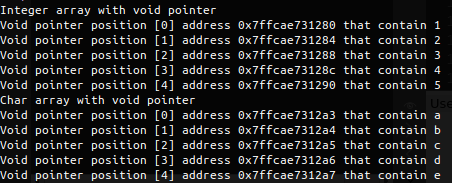
\includegraphics[scale=0.5]{screens/screen1.png}\\
\textit{Output del código de ejemplo 3}
\end{center}
Ahora que pasa si por error o juego se hace otro tipo de casting del arreglo.
\lstinputlisting[language=C]{./sourceCodes/violatePointer2.c}
\begin{center}
\textit{Código fuente 4}\\
\end{center}
\begin{center}
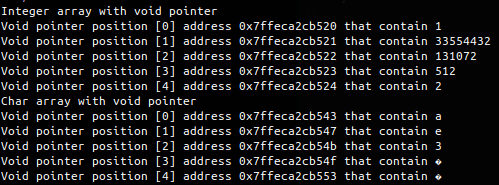
\includegraphics[scale=0.5]{screens/screen2.png}\\
\textit{Output del código de ejemplo 4}
\end{center}
Esto puede significar que se puede romper o en su defecto realizar operaciones que "no esten permitidas en el lenguaje", pero que dentro de su sintaxis y de la misma curiosidad del programador este puede abusar del movimiento de direcciones y del tipo de casting que existe en el lenguaje.
\section{Apuntadores de varias dimensiones}
Si bien el hacer uso de apuntadores permite el manejo inteligente de sus variables y de memoria dínamica con apuntadores simples, ahora que pasa cuando se hace en varias dimensiones de apuntador, es decir, que se haga varios apuntadores "*"
\subsection{Ejemplo con apuntadores dobles}
\lstinputlisting[language=C]{./sourceCodes/apuntadordoble.c}
\begin{center}
\textit{Código fuente 5}\\
\end{center}
\lstinputlisting[language=C]{./sourceCodes/matriz.c}
\begin{center}
\textit{Código fuente 6}\\
\end{center}
\subsection{Ejemplo con apuntadores de más de dos dimensiones}

\lstinputlisting[language=C]{./sourceCodes/volumen.c}
\begin{center}
\textit{Código fuente 7}\\
\end{center}

\section{Estructura de datos}
Una estructura es una colección de datos, en el no solo contiene datos, sino que igual que contiene una serie de operaciones, en algunos casos un ejemplo en el que se puede trabajar esto es con números complejos, que si bien es claro en algunos lenguajes no esta definido este tipo de dato.
\lstinputlisting[language=C]{./sourceCodes/complex.c}
\begin{center}
\textit{Código fuente 8}\\
\end{center}

\section{Recursividad}
Es una entidad que se define en términos de sí mismas, en algunos casos de ellos es:
\begin{itemize}
  \item Arboles
  \item Celulas
  \item Fractales
  \item Sistemas formales matemáticos
  \item Computación
  \begin{enumerate}
    \item Automatización
    \item Máquina de Turing (Máquina Universal)
    \begin{itemize}
      \item Estados: $\mathcal{Q}$
      \item Configuraciones: $\mathsf{M}$
      \item Transiciones: $\delta$
      \item Estado inicial: $\mathsf{q0}$
      \item Estado final: $\mathsf{qf}$
    \end{itemize}
    \item Lenguaje que puede ser recursivamente enumerable: $\mathcal{L}$
    \item Contiene palabras del Lenguaje $\mathcal{L}$ que pueden mapearse al conjunto $\mathbb{N}$
  \end{enumerate}
\end{itemize}
Un ejemplo de código con recursividad es el siguiente:
\lstinputlisting[language=C]{./sourceCodes/eternalLoop.c}
\begin{center}
\textit{Código fuente 9}\\
\end{center}
Si este es ejecutado dependiendo el sistema operativo puede acabar o no
\begin{center}
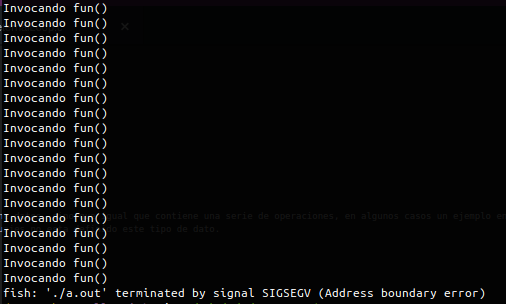
\includegraphics[scale=0.5]{screens/screen3.png}\\
\textit{Output del código de ejemplo 9\\Ejecutado en un sistema operativo Linux}
\end{center}
Llevando acabo un contador como en la siguiente forma:
\lstinputlisting[language=C]{./sourceCodes/eternalLoop2.c}
\begin{center}
\textit{Código fuente 10}\\
\end{center}
Si este es ejecutado dependiendo el sistema operativo puede acabar o no
\begin{center}
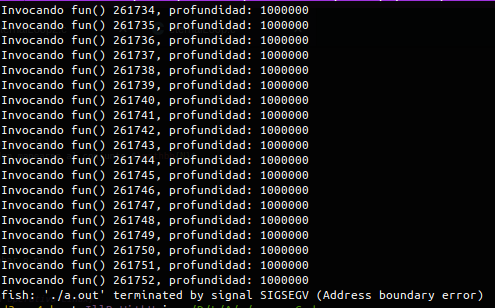
\includegraphics[scale=0.5]{screens/screen4.png}\\
\textit{Output del código de ejemplo 10\\Ejecutado en un sistema operativo Linux}
\end{center}
En algunos casos dependiendo la planificación del sistema operativo, como el hardware del equipo y versión del compilador puede que vaya hasta el final o se pare en otra posición de donde se rompa la recursividad
\lstinputlisting[language=C]{./sourceCodes/eternalLoop3.c}
\begin{center}
\textit{Código fuente 11}\\
\end{center}
Ejecutando este programa a 5 niveles tenemos
\begin{center}
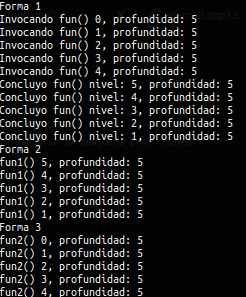
\includegraphics[scale=0.5]{screens/screen5.png}\\
\textit{Output del código de ejemplo 11}
\end{center}
Otra forma de ver la idea del codigo anterior implementada de distinta forma es
\lstinputlisting[language=C]{./sourceCodes/recursividad.c}
\begin{center}
\textit{Código fuente 12}\\
\end{center}
Ahora a continuación se presentara finalmente dos aplicaciones interesantes de la recursividad en dos problemas que computacionalmente se abordan en clases (en el mejor de los casos).
\\
\subsection{Torres de hanoi}
Este es un problema que se puede resolver computacionalmente que puede ser presentado en tres torres la cual consta de mover N cantidad de aros hasta la ultima torre, para un efecto ilustrativo aquí esta un link con información: \href{https://www.youtube.com/watch?v=LM68IQvIo_E}{\underline{Vídeo}}
\lstinputlisting[language=C]{./sourceCodes/hanoi.c}
\begin{center}
\textit{Código fuente 13}\\
\end{center}
\subsection{Problema de las 8 reinas}
Es un problema que trata de acomodar 8 reinas o n reinas dependiendo el caso en un tablero de 8*8 o n*n segun el caso respectivamente de tal forma en la que cada reina no se toque, para más información esta \href{https://www.youtube.com/watch?v=WOZ4wDt-iYA}{\underline{Vídeo}}
\lstinputlisting[language=C]{./sourceCodes/8reinas.c}
\begin{center}
\textit{Código fuente 13}\\
\end{center}
\begin{center}
\textbf{Gracias}\\
\end{center}
\printindex
\end{document}
